\section{Das zweite Deformationslemma}

\begin{theorem}[Zweites Deformations-Lemma]
    \label{theorem:zweites deformationslemma}
    Es sei $M$ eine glatte Mannigfaltigkeit, $f: M \rightarrow \R$ eine glatte
    Abbildung und $p$ ein nicht-degenerierter kritischer Punkt mit Index 
    $k$. Sei $c := f(p)$ und $\varepsilon \geq 0$, sd. 
    $f^{-1}[c - \varepsilon, c + \varepsilon]$ kompakt ist und außer $p$ keine 
    weiteren kritischen Punkte von $f$ beinhaltet. Dann hat $M^{c-\varepsilon}$
    denselben Homotopietypen wie $M^{c - \varepsilon} \cup e^k$.
\end{theorem}

Das ist die zweite Aussage, die wir am Anfang am Beispiel des Torus beobachtet haben!

Die Idee für den Beweis ist, sich eine neue Funktion $F: M \to \R$ zu definieren,
die Außerhalb von einer kleinen Umgebung von $p$ $f$ entspricht und in der 
Umgebung etwas kleiner ist. Dann bekommen wir die folgende Situation:

\begin{figure}[H]
    \centering
    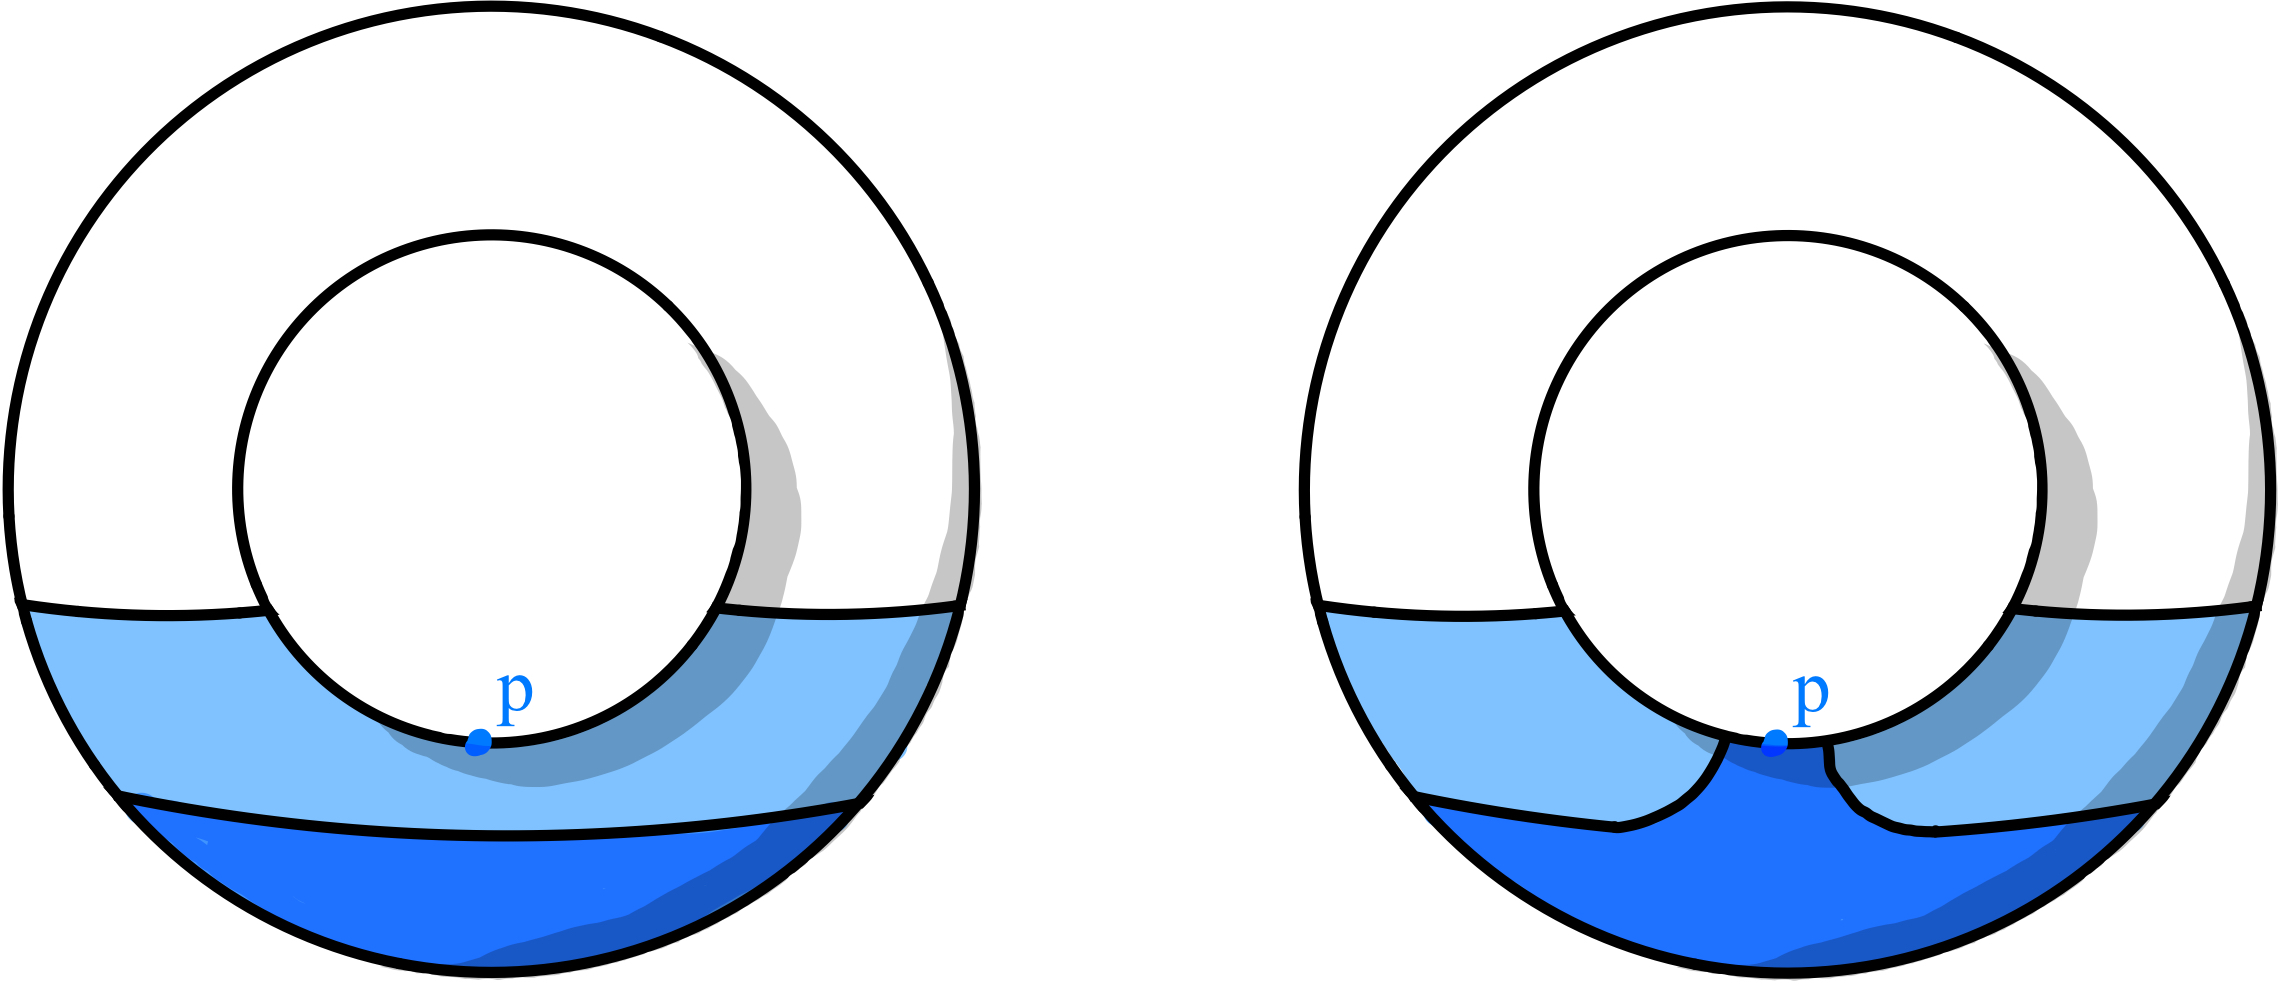
\includegraphics[width=0.8\linewidth]{resources/Me-Diagram5-sublevelsets-of-f-and-F.jpeg}
    \label{fig:me-diagram5}
    \caption{Die Niveaumengen von $f$ (links) und $F$ (rechts)}
\end{figure}

Wir wollen also, dass $M^{c + \varepsilon} = F^{-1}(- \infty, c + \varepsilon]$ 
gilt und $F^{-1}(-\infty, c - \varepsilon]$ fast dasselbe ist wie 
$M^{c - \varepsilon}$, nur dass $F^{-1}(-\infty, c - \varepsilon]$ einen "Henkel"
enthält der den kritischen Punkt $p$ enthält.

\begin{proof}[Beweis zweites Deformationslemma]
    Sei $c := f(p)$. Mit dem Morse-Lemma können wir lokale Koordinaten 
    $(u_1, ..., u_n)$ in einer Umgebung $U$ von $p$ wählen, sodass
    \[ f = c - u_1^2 - ... - u_k^2 + u_{k+1}^2 + ... + u_n^2 \]
    in dieser Umgebung, und sodass für den kritischen Punkt $p$ gilt:
    \[ u_1(p) = ... = u_n(p) = 0 \]

    Sei oBdA $\varepsilon > 0$ klein genug, sodass 
    \begin{enumerate}
        \item $f^{-1}[c - \varepsilon, c + \varepsilon]$ kompakt ist und keine
            kritischen Punkte außer $p$ enthält
        \item $\{ x \in \R^n: \lVert x \rVert^2 \leq 2 \varepsilon \} \subseteq \varphi(U) $
    \end{enumerate}

    Wähle nun die $k$-Zelle 
    \[ 
        e^k := \{ p \in M: (u_1(p))^2 + ... + (u_k(p))^2 \leq \varepsilon 
        \text{ und } u_{k+1}(p) = ... = u_n(p) = 0 \} 
    \]

    Wir bekommen die folgende Situation:

    \begin{figure}[H]
        \centering
        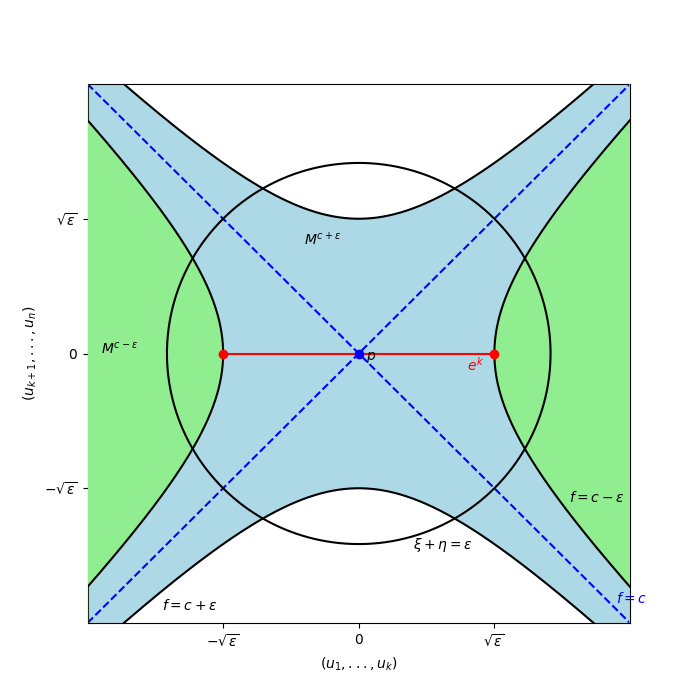
\includegraphics[width=0.8\linewidth]{resources/Me-Diagram6-U-parameterized.png}
        \label{fig:me-diagram6}
        \caption{U parametrisiert}
    \end{figure}

    Nun definiere eine glatte Funktion $\mu: \R \to \R$ mit den Eigenschaften:

    \begin{enumerate}
        \item $ \mu(0) > \varepsilon $
        \item $ \mu(r) = 0 $ falls $ r \geq 2 \varepsilon $
        \item $ -1 < \mu'(r) \leq 0 $ für alle $ r \in \R $
    \end{enumerate}

    Sei nun $F$ außerhalb von $U$ gleich $f$, und sei
    \[ F = f - \mu(u_1^2 + ... + u_k^2 + 2u_{k+1}^2 + ... + 2u_n^2) \]

    $F$ ist wohldefiniert und glatt, da $F$ außerhalb des Kreises mit Radius 
    $\sqrt{2\varepsilon}$ mit $f$ übereinstimmt und der gesamte Kreis in $U$ 
    enthalten ist. Damit haben wir einen guten Kandidaten foür $F$ gefunden.

    Wir definieren nun

    \begin{align*}
        & \eta, \xi: U \to [0, \infty) \\
        & \xi = u_1^2 + ... + u_k^2 \\
        & \eta = u_{k + 1}^2 + ... + e_n^2
    \end{align*}

    Dann gilt innerhalb von $U$:
    \[ f = c - \xi + \eta \]
    und 
    \[ F = f - \mu(\xi + 2 \eta) = c - \xi + \eta - \mu(\xi + 2 \eta) \]

    Jetzt wollen wir überprüfen:
    \begin{enumerate}
        \item $F^{-1}(-\infty, c + \varepsilon] = M^{c + \varepsilon}$.
        \item $F^{-1}(-\infty, c - \varepsilon]$ ist ein Deformationsretrakt von 
            $M^{c + \varepsilon}$.
        \item $M^{c - \varepsilon} \cup e^k$ ist ein Deformationsretrakt von
            $F^{-1}(-\infty, c - \varepsilon]$.
    \end{enumerate}

    Dann folgt schon die Behauptung.

    \proofheading{Behauptung 1} $F^{-1}(-\infty, c + \varepsilon] = M^{c + \varepsilon}$

    Sei $q \in M$. Falls gilt $\xi(q) + 2 \eta(q) > 2 \varepsilon$ gilt 
    $F(q) = f(q) - \mu(\xi(q) + 2\eta(q)) = f(q)$,
    also gelte oBdA 
    \[ \xi(q) + 2 \eta(q) \leq 2 \varepsilon \]
    Dann:
    \[ F(q) \leq f(q) = c - \xi(q) + \eta(q) \leq c + \frac{1}{2}\xi(q) + \eta(q) \leq c + \varepsilon \]
    \sectiondone

    \proofheading{Behauptung 2} $F^{-1}(-\infty, c - \varepsilon]$ ist ein
    Deformationsretrakt von $M^{c + \varepsilon}$.

    Bemerke: Die kritischen Punkte von $F$ stimmen mit denen von $f$ überein, 
    denn:

    \[ \pderive[F]{\xi} = -1 - \mu'(\xi + 2\eta)  < 0 \]
    und
    \[ \pderive[F]{\eta} = 1 - 2 \mu'(\xi + 2\eta) \geq 1 \]
    Insbsondere sind diese beiden Ableitungen also niemals $0$. Da 
    \[ \opd F = \pderive[F]{\xi}\opd \xi + \pderive[F]{\eta} \opd \eta \]
    und $\opd \xi$ und $\opd \eta$ nur in $p$ gleichzeitig Null sind, haben $f$ 
    und $F$  dieselben kritischen Punkte.

    Betrachte die Region $F^{-1}[c - \varepsilon, c + \varepsilon]$. Wegen 
    Behauptung 1 und der Tatsache, dass $F \leq f$ gilt:
    \[ F^{-1}[c - \varepsilon, c + \varepsilon] \subseteq f^{-1}[c - \varepsilon, c + \varepsilon] \]
    Da $f^{-1}[c - \varepsilon, c + \varepsilon]$ kompakt ist und 
    $F^{-1}[c - \varepsilon, c + \varepsilon]$ abgeschlossen ist, ist 
    $F^{-1}[c - \varepsilon, c + \varepsilon]$ auch kompakt. Da $f$ und $F$
    dieselben kritischen Punkte haben kann diese Menge maximal den kritischen 
    Punkt $p$ enthalten, aber
    \[ F(p) = c - \mu(0) < c - \varepsilon \]
    Also gibt es in $F^{-1}[c - \varepsilon, c + \varepsilon]$ keine kritischen
    Punkte. Mit dem ersten Deformationslemma gilt dann:
    $F^{-1}(- \infty, c - \varepsilon]$ ist Def. Retrakt von 
    $F^{-1}(-\infty, c + \varepsilon] = M^{c + \varepsilon}$.
    \sectiondone

    \proofheading{Behauptung 3} $M^{c - \varepsilon} \cup e^{k}$ ist ein 
    Deformationsretrakt von $F^{-1}(-\infty, c - \varepsilon]$.

    Diese Aussage ergibt nur Sinn, falls 
    $M^{c - \varepsilon} \cup e^{k} \subseteq F^(-\infty, c - \varepsilon]$.
    Wir wissen schon, dass $M^{c - \varepsilon} \subseteq F^{-1}(c - \varepsilon]$.

    Sei $q \in e^k$, dann gilt $\xi(p) = 0 \leq \xi(q) \leq 1$. Da 
    $\pderive[F]{\xi} < 0$, gilt dann
    \[ F(q) \leq F(p) = c - \xi(p) + \eta(p) + \mu(\xi(p) + 2\eta(p)) = c - \mu(0) \leq c - \varepsilon \]

    Also ergibt sich folgende Situation:

    \begin{figure}[H]
        \centering
        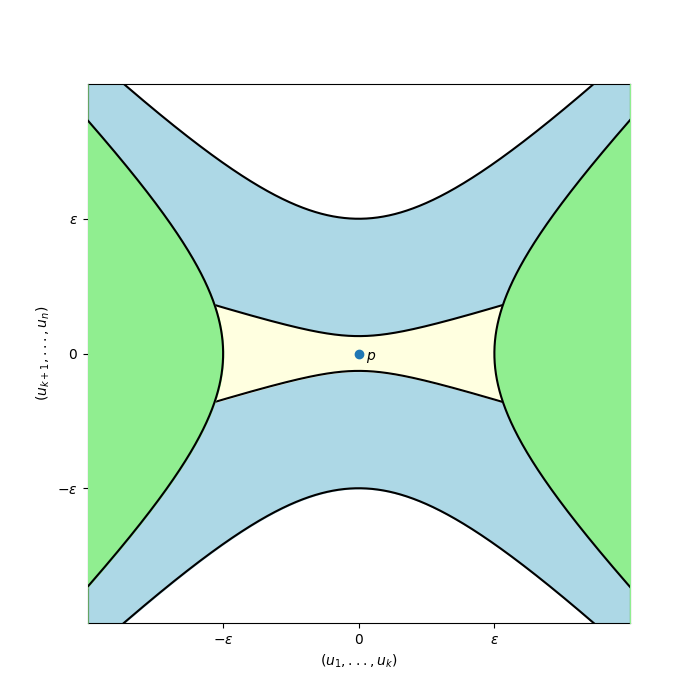
\includegraphics[width=0.8\linewidth]{resources/Me-Diagram7-handle.png}
        \label{fig:me-diagram7}
        \caption{Henkel}
    \end{figure}

    Die hellgrün eingefärbte Fläche ist $M^{c - \varepsilon}$ die hellgelbe
    zusammen mit der hellgrünen Fläch ist $F^{-1}(-\infty, c - \varepsilon]$. 

    Dafür konstruieren wir eine Deformationsretraktion
    $r: M^{c - \varepsilon} \cup H \times [0,1] \to M^{c - \varepsilon} \cup H$
    für $q \in M^{c - \varepsilon} \cup H, t \in [0, 1]$, die $H$ auf $e^k$ 
    deformiert, wie folgt.

    \[
        r(q, t) = \begin{cases}
            \varphi^{-1} \circ (u_1, ..., u_k, tu_{k + 1}, ..., tu_n)(q)
                & \text{ im Fall 1: } \xi(q) \leq \varepsilon \\
            \varphi^{-1} \circ (u_1, ..., u_k, s_tu_{k + 1}, ..., s_tu_n)(q)
                & \text{ im Fall 2: } \varepsilon \leq \xi(q) \leq \eta(q) + \varepsilon \\
            q & \text{ im Fall 3: } \eta(q) + \varepsilon \leq \xi(q)
        \end{cases}
    \]

    Wobei 

    \[ s_t = t + (1 -t)((\xi - \varepsilon)/\eta)^{1/2} \]

    Die Fälle sind dann wie folgt:

    \begin{figure}[H]
        \centering
        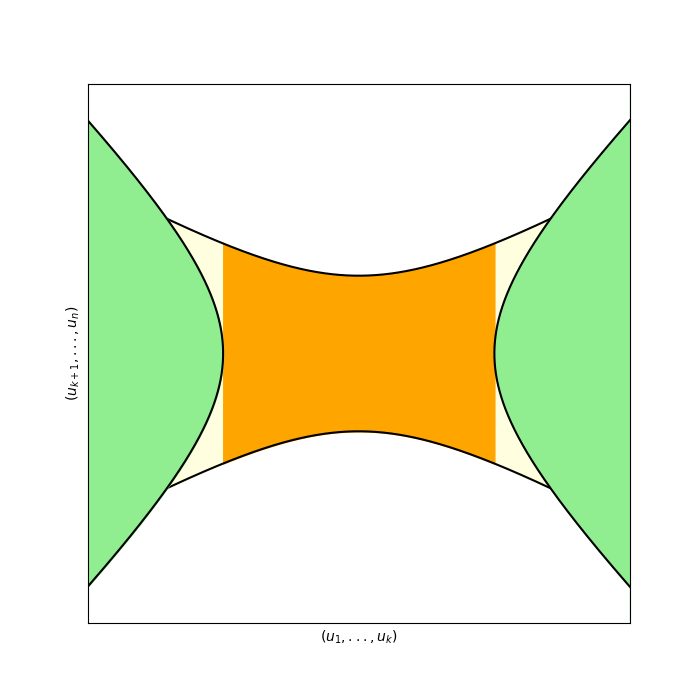
\includegraphics[width=0.8\linewidth]{resources/Me-Diagram9-handle-cases.png}
        \label{me-diagram9}
        \caption{
            Fall 3 ist $M^{c - \varepsilon}$, also die grün eingefärbte Fläche, die
            orangene Fläche ist Fall 1 und die gelbe ist Fall 2.
        }
    \end{figure}

    Wir müssen überprüfen:
    \begin{enumerate}
        \item $r$ ist wohldefiniert und stetig
        \item $r(M^{c - \varepsilon} \cup H, 0) \subseteq M^{c - \varepsilon} \cup e^k$
        \item $r(\cdot, 1) = \id_{M^{c - \varepsilon} \cup H}$ und 
            $\left. r(\cdot , 0) \right\vert_{M^{c - \varepsilon} \cup e^k} 
            = \id_{M^{c - \varepsilon} \cup e^k}$
    \end{enumerate}

    3. ist einfach nachzurechnen. In Fall 1 und Fall 3 ist 2. offensichtlich
    wahr. Für Fall 2 gilt:
    \begin{align*} 
        f(r(0, q)) & = 
            f\left( \varphi^{-1} \left(u_1(q), ..., u_k(q), 
            \left( \frac{\xi(q) - \varepsilon}{\eta(q)} \right)^{1/2}u_{k + 1}(q), ...,
            \left( \frac{\xi(q) - \varepsilon}{\eta(q)} \right)^{1/2}u_n(q)
            \right)
            \right) \\
        & = c - \xi(q)
            + \left( \left( \frac{\xi(q) - \varepsilon}{\eta(q)} \right)^{1/2}u_{k + 1}(q) \right)^2 + ... 
            + \left( \left( \frac{\xi(q) - \varepsilon}{\eta(q)} \right)^{1/2}u_n(q) \right)^2 \\
        & = c - \left( \frac{\xi(q) - \varepsilon}{\eta(q)} \right) \eta(q) \\
        & = c - \varepsilon
    \end{align*}
    also ist $r(0, q) \in f^{-1}(c - \varepsilon)$. Um 1. zu prüfen müssen wir 
    Stetigkeit in den Grenzfällen überprüfen:
    \begin{align*}
        & \text{For } \xi(q) = \varepsilon \text{ : }
            & s_t(q)  =t + (1 - t)((\varepsilon - \varepsilon)/\eta(q))^{1/2} = t \\
        & \text{For } \eta(q) + \varepsilon = \xi(q) \text{ : }
            & s_t(q) = t + (1 - t)((\xi(q) - \varepsilon)/(\xi(q) - \varepsilon))^{1/2} = 1
    \end{align*}

    Das einzig andere Problem was wir bekommen könnten ist nun in Fall 2 falls
    $\eta \to 0$. In Fall 1 und Fall 3 bekommen wir für $q$ mit $\eta(q) = 0$:
    $r(q, t) = \varphi^{-1} \circ (u_1, ..., u_k, 0, ..., 0)(q)$, also wollen
    wir zeigen dass für $\eta \in $ Fall 2 mit $\eta \to 0$ gilt $s_tu_i \to 0$
    für $i \in \{k+1, ..., n\}$. In Fall 2 gilt
    $0 \leq \xi - \varepsilon \leq \eta$. Dann gilt:

    \begin{align*}
        \lim\limits_{\eta \to 0} | s_t u_i |
           & = \lim\limits_{\eta \to 0} (1 - t)((\xi - \varepsilon)/\eta)^{1/2} | u_i | \\
           & \leq \lim\limits_{\eta \to 0} (1 - t)(\eta/\eta)^{1/2}|u_i| \\
           & = \lim\limits_{\eta \to 0} (1 - t)|u_i| = 0 
    \end{align*}
    
    Also ist $r$ stetig.
    \sectiondone

    Mit Behauptung 3 und 4 bekommen wir
    \[ M^{c + \varepsilon} \simeq F^{-1}(c - \varepsilon] \]
    und 
    \[ F^{-1}(-\infty, c - \varepsilon] \simeq M^{c - \varepsilon} \cup e^k \]
    Also folgt die Behauptung:
    \[ M^{c + \varepsilon} \simeq M^{c - \varepsilon} \cup e^k \]

\end{proof}

\begin{corollary}
    Allgemeiner gilt sogar: Angenommen es gibt $m$ kritische Punkte 
    $p_1, ..., p_m$ mit Indizes $k_1, ..., k_m$ in $f^{-1}(c)$. Dann gilt
    \[ M^{c + \varepsilon} \simeq M^{c - \varepsilon} \cup e^{k_1} \cup ... \cup e^{k_m} \]

    Die Anheftungssabbildungen können hier so gewählt werden, dass ihre Bilder 
    disjunkt in $M^{c + \varepsilon}$ liegen, also funktioniert hier unsere 
    ursprüngliche Definition vom Anheften einer $k$-Zelle noch immer.
\end{corollary}
